% -*- coding: utf-8 -*-
% LuaLaTeX 用ドキュメント
% コンパイル: lualatex DenseLinear.tex

\documentclass[a4paper,11pt]{ltjsarticle}

% LuaTeX-ja 設定
\usepackage{luatexja}
\usepackage{luatexja-fontspec}

% 数学関連
\usepackage{amsmath,amssymb,amsthm}
\usepackage{mathtools}

% 図式・TikZ
\usepackage{tikz}
\usetikzlibrary{arrows.meta,positioning,calc,decorations.pathreplacing,shapes.geometric,patterns}
\usepackage{tikz-cd}

% ハイパーリンク
\usepackage{hyperref}
\hypersetup{
    colorlinks=true,
    linkcolor=blue!70!black,
    urlcolor=blue!50!black
}

% コード表示
\usepackage{listings}
\lstset{
    basicstyle=\ttfamily\small,
    keywordstyle=\color{blue!80!black}\bfseries,
    commentstyle=\color{green!50!black}\itshape,
    stringstyle=\color{red!70!black},
    frame=single,
    breaklines=true,
    numbers=left,
    numberstyle=\tiny\color{gray},
    xleftmargin=2em,
    framexleftmargin=1.5em,
    backgroundcolor=\color{gray!5}
}

% 色
\usepackage{xcolor}

% 定理環境
\theoremstyle{definition}
\newtheorem{definition}{定義}[section]
\newtheorem{example}[definition]{例}

\theoremstyle{plain}
\newtheorem{theorem}[definition]{定理}
\newtheorem{proposition}[definition]{命題}
\newtheorem{lemma}[definition]{補題}
\newtheorem{corollary}[definition]{系}

\theoremstyle{remark}
\newtheorem{remark}[definition]{注意}
\newtheorem{insight}[definition]{知見}

% カスタムコマンド
\newcommand{\Q}{\mathbb{Q}}
\newcommand{\N}{\mathbb{N}}
\newcommand{\Layer}{\mathrm{layer}}
\newcommand{\minLayer}{\mathrm{minLayer}}

% タイトル
\title{%
    \textbf{稠密線形順序と最小層の不存在}\\[0.5em]
    \Large Dense Linear Order and Non-existence of Minimum Layer
}

\author{su\thanks{Lean ソースコードおよび本 \TeX 文書ともに AI ツール Antigravity (Google DeepMind) を使用して作成しました。}}

\date{2025年12月28日}

\begin{document}

\maketitle

\begin{abstract}
本文書は、構造塔理論において「線形順序だけでは $\minLayer$ の well-definedness には不十分である」
ことを示す反例 \texttt{denseLinearNoLeast} を数学的に解説する。
添字集合として有理数 $\Q$ を用い、被覆性・単調性が成立するにもかかわらず、
点 $0$ に対して最小層が存在しないことを Lean 4 で形式化した。
\end{abstract}

\tableofcontents

\newpage

%=============================================================================
\section{背景と動機}
%=============================================================================

構造塔理論において、$\minLayer$ の well-definedness を保証する条件として
「添字集合が線形順序であること」がしばしば主張される。しかし、これは
\textbf{必要条件として不十分}であることが、以下の反例によって示される。

\begin{insight}[線形順序だけでは不十分]
添字集合 $(I, \leq)$ が線形順序（全順序）であっても、稠密順序の場合には
$S_x := \{i \in I \mid x \in \Layer(i)\}$ が最小元を持たない可能性がある。
\end{insight}

本稿では、$I = \Q$（有理数）を添字とする具体例を構成し、この知見を証明する。

%=============================================================================
\section{構成：稠密線形順序塔}
%=============================================================================

\begin{definition}[稠密線形順序塔]
以下のデータで構造塔を定義する：
\begin{align*}
    X &= \Q \\
    I &= \Q \quad (\Q \text{ の通常の順序}) \\
    \Layer(q) &= \{x \in \Q \mid x < q\}
\end{align*}
\end{definition}

\begin{figure}[htbp]
\centering
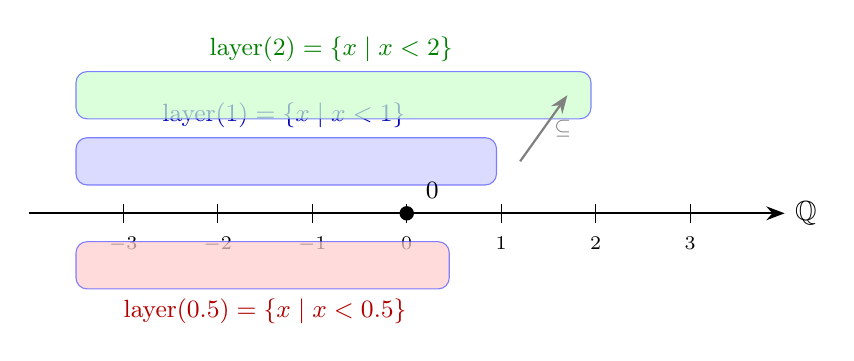
\begin{tikzpicture}[
    scale=1.2,
    layer/.style={draw=blue!70, fill=blue!10, rounded corners},
    pt/.style={circle, draw=black!70, fill=green!30, minimum size=0.4cm, font=\scriptsize},
    axis/.style={-Stealth, thick}
]

% 数直線
\draw[axis] (-4, 0) -- (4, 0) node[right] {$\Q$};

% 目盛り
\foreach \x in {-3,-2,-1,0,1,2,3} {
    \draw (\x, -0.1) -- (\x, 0.1);
    \node[below, font=\scriptsize] at (\x, -0.15) {$\x$};
}

% layer(1) の図示
\draw[layer, fill=blue!20, opacity=0.7] (-3.5, 0.3) rectangle (0.95, 0.8);
\node[above, font=\small, blue!70!black] at (-1.3, 0.8) {$\Layer(1) = \{x \mid x < 1\}$};

% layer(2) の図示
\draw[layer, fill=green!20, opacity=0.7] (-3.5, 1.0) rectangle (1.95, 1.5);
\node[above, font=\small, green!50!black] at (-0.8, 1.5) {$\Layer(2) = \{x \mid x < 2\}$};

% layer(0.5) の図示
\draw[layer, fill=red!20, opacity=0.7] (-3.5, -0.8) rectangle (0.45, -0.3);
\node[below, font=\small, red!70!black] at (-1.5, -0.8) {$\Layer(0.5) = \{x \mid x < 0.5\}$};

% 0 の位置
\filldraw[black] (0, 0) circle (2pt);
\node[above right, font=\small] at (0.1, 0.05) {$0$};

% 矢印で包含関係
\draw[-Stealth, thick, gray] (1.2, 0.55) -- (1.7, 1.25) node[midway, right, font=\scriptsize] {$\subseteq$};

\end{tikzpicture}
\caption{稠密線形順序塔：$\Layer(q) = \{x \mid x < q\}$}
\label{fig:dense-layer}
\end{figure}

\begin{remark}
直感的には、$\Layer(q)$ は数直線上で $q$ より左側の領域全体を表す。
$q$ が大きくなるほど $\Layer(q)$ も大きくなる（単調性）。
\end{remark}

%=============================================================================
\section{公理の検証}
%=============================================================================

\subsection{被覆性}

\begin{theorem}[被覆性の成立]
任意の $x \in \Q$ に対して、$x \in \Layer(q)$ となる $q \in \Q$ が存在する。
\end{theorem}

\begin{proof}
$q = x + 1$ とすれば、$x < x + 1 = q$ なので $x \in \Layer(q)$。
\end{proof}

\begin{figure}[htbp]
\centering
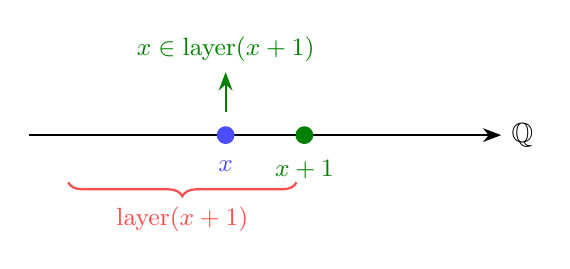
\begin{tikzpicture}[
    scale=1.0,
    axis/.style={-Stealth, thick}
]

% 数直線
\draw[axis] (-1, 0) -- (5, 0) node[right] {$\Q$};

% x の位置
\filldraw[blue!70] (1.5, 0) circle (3pt);
\node[below, font=\small, blue!70] at (1.5, -0.2) {$x$};

% x+1 の位置
\filldraw[green!50!black] (2.5, 0) circle (3pt);
\node[below, font=\small, green!50!black] at (2.5, -0.2) {$x+1$};

% layer(x+1) の範囲
\draw[thick, red!70, decorate, decoration={brace, amplitude=5pt, mirror}] 
    (-0.5, -0.6) -- (2.4, -0.6) node[midway, below=5pt, font=\small] {$\Layer(x+1)$};

% x が含まれる
\draw[-Stealth, thick, green!50!black] (1.5, 0.3) -- (1.5, 0.8) 
    node[above, font=\small] {$x \in \Layer(x+1)$};

\end{tikzpicture}
\caption{被覆性：$x \in \Layer(x+1)$}
\label{fig:covering}
\end{figure}

\subsection{単調性}

\begin{theorem}[単調性の成立]
$p \leq q$ ならば $\Layer(p) \subseteq \Layer(q)$。
\end{theorem}

\begin{proof}
$x \in \Layer(p)$ とすると $x < p$。$p \leq q$ より $x < q$ なので $x \in \Layer(q)$。
\end{proof}

%=============================================================================
\section{最小層の不存在}
%=============================================================================

\subsection{$S_0$ の定義と性質}

\begin{definition}[$S_x$ の定義]
点 $x \in X$ に対して、$x$ が属する層の添字集合を次で定義する：
\[
    S_x := \{q \in \Q \mid x \in \Layer(q)\}
\]
\end{definition}

\begin{proposition}[$S_0$ の特徴付け]
$S_0 = \{q \in \Q \mid 0 < q\} = \Q_{>0}$（正の有理数全体）。
\end{proposition}

\begin{proof}
$0 \in \Layer(q) \Leftrightarrow 0 < q$ より自明。
\end{proof}

\subsection{最小元の不存在}

\begin{theorem}[$S_0$ に最小元は存在しない]\label{thm:no-least}
$S_0 = \Q_{>0}$ は最小元を持たない。
\end{theorem}

\begin{figure}[htbp]
\centering
\begin{tikzpicture}[
    scale=1.5,
    axis/.style={-Stealth, thick},
    pt/.style={circle, draw=black!70, fill=red!30, minimum size=0.35cm, font=\scriptsize}
]

% 数直線
\draw[axis] (-0.5, 0) -- (4, 0) node[right] {$\Q_{>0}$};

% 0 の位置（白抜き）
\draw[thick] (0, 0) circle (2pt);
\node[below, font=\small] at (0, -0.15) {$0$};

% 候補 m
\filldraw[red!70] (2, 0) circle (3pt);
\node[above, font=\small, red!70] at (2, 0.15) {$m$};

% m/2
\filldraw[blue!70] (1, 0) circle (3pt);
\node[above, font=\small, blue!70] at (1, 0.15) {$\frac{m}{2}$};

% m/4
\filldraw[green!50!black] (0.5, 0) circle (3pt);
\node[above, font=\small, green!50!black] at (0.5, 0.15) {$\frac{m}{4}$};

% m/8
\filldraw[orange!70] (0.25, 0) circle (3pt);
\node[above, font=\scriptsize, orange!70] at (0.25, 0.2) {$\frac{m}{8}$};

% 矢印で「より小さい元がある」
\draw[-Stealth, thick, gray] (2, -0.3) to[bend right=20] node[below, font=\scriptsize] {$<$} (1, -0.3);
\draw[-Stealth, thick, gray] (1, -0.3) to[bend right=20] node[below, font=\scriptsize] {$<$} (0.5, -0.3);
\draw[-Stealth, thick, gray] (0.5, -0.3) to[bend right=20] node[below, font=\scriptsize] {$<$} (0.25, -0.3);

% 省略記号
\node at (0.1, -0.5) {$\cdots$};

% 注釈
\node[text width=5cm, align=left, font=\small] at (5.5, 0) {
    どんな $m > 0$ を取っても\\
    $\frac{m}{2} \in S_0$ かつ $\frac{m}{2} < m$\\[0.5em]
    $\Rightarrow$ 最小元は存在しない
};

\end{tikzpicture}
\caption{$S_0 = \Q_{>0}$ に最小元がないことの図解}
\label{fig:no-least}
\end{figure}

\begin{proof}
背理法で示す。$m \in S_0$ が最小元であると仮定する。

$m \in S_0$ より $0 < m$。ここで $\frac{m}{2}$ を考えると：
\begin{enumerate}
    \item $0 < \frac{m}{2}$ なので $\frac{m}{2} \in S_0$
    \item $\frac{m}{2} < m$
\end{enumerate}
$m$ が最小元ならば $m \leq \frac{m}{2}$ でなければならないが、これは $\frac{m}{2} < m$ と矛盾する。
\end{proof}

\begin{corollary}[$\minLayer(0)$ は well-defined でない]
$0 \in \Q$ に対して、最小層 $\minLayer(0)$ は存在しない。
\end{corollary}

\begin{proof}
$\minLayer(0)$ が存在するとすれば、それは $S_0$ の最小元である。
しかし定理~\ref{thm:no-least} より $S_0$ に最小元は存在しない。
\end{proof}

%=============================================================================
\section{稠密性の本質的役割}
%=============================================================================

\begin{figure}[htbp]
\centering
\begin{tikzpicture}[
    order/.style={draw=blue!70!black, thick, rounded corners=8pt, fill=blue!10, 
                  minimum width=3.5cm, minimum height=1.5cm, align=center},
    ok/.style={-Stealth, thick, green!50!black},
    ng/.style={-Stealth, thick, red!60, dashed}
]

% 3種類の順序
\node[order] (wo) at (0, 0) {\textbf{整列集合}\\（例：$\N$）};
\node[order] (dense) at (5, 0) {\textbf{稠密線形順序}\\（例：$\Q$）};
\node[order] (po) at (10, 0) {\textbf{半順序}\\（例：$\N \times \N$）};

% 結果
\node[green!50!black, font=\small, align=center] at (0, -1.8) {$\minLayer$ は\\well-defined};
\node[red!60, font=\small, align=center] at (5, -1.8) {$\minLayer$ は\\well-defined でない\\（最小元なし）};
\node[red!60, font=\small, align=center] at (10, -1.8) {$\minLayer$ は\\well-defined でない\\（比較不能）};

% 矢印
\draw[ok] (wo.south) -- (0, -1.2);
\draw[ng] (dense.south) -- (5, -1.2);
\draw[ng] (po.south) -- (10, -1.2);

% タイトル
\node[font=\bfseries\large] at (5, 2) {添字順序の比較};

% 失敗の原因
\node[font=\scriptsize, gray] at (5, -2.8) {稠密性により常により小さい元が存在};
\node[font=\scriptsize, gray] at (10, -2.8) {比較不能な元が存在};

\end{tikzpicture}
\caption{添字順序と $\minLayer$ の well-definedness}
\label{fig:order-comparison}
\end{figure}

\begin{insight}[整列性の必要性]
$\minLayer$ が well-defined であるためには、添字集合 $(I, \leq)$ が単なる線形順序では不十分であり、
各 $S_x$ が最小元を持つこと、すなわち $(I, \leq)$ が整列集合（または同等の条件）であることが必要である。
\end{insight}

%=============================================================================
\section{Lean 実装}
%=============================================================================

本稿の内容は、以下の Lean 4 コードで形式化されている。

\begin{lstlisting}[language=ML, caption={denseLinearLayer の定義}]
def denseLinearLayer (q : Q) : Set Q := {x | x < q}
\end{lstlisting}

\begin{lstlisting}[language=ML, caption={$S_0$ に最小元がないことの証明}]
theorem S_zero_has_no_least : 
    ¬ exists m : Q, m ∈ S_zero ∧ ∀ q ∈ S_zero, m ≤ q := by
  intro ⟨m, hm_in, hm_least⟩
  rw [S_zero_eq] at hm_in hm_least
  simp only [mem_setOf_eq] at hm_in hm_least
  have h_half_pos : (0 : Q) < m / 2 := by linarith
  have h_contra : m ≤ m / 2 := hm_least (m / 2) h_half_pos
  linarith
\end{lstlisting}

%=============================================================================
\section{結論}
%=============================================================================

本稿では、稠密線形順序 $\Q$ を添字とする構造塔において、
被覆性・単調性が成立するにもかかわらず $\minLayer$ が well-defined にならないことを示した。

\begin{table}[htbp]
\centering
\caption{denseLinearNoLeast の公理成立状況}
\small
\begin{tabular}{|l|c|l|}
\hline
\textbf{公理} & \textbf{成立} & \textbf{備考} \\
\hline
被覆性 & $\checkmark$ & $x \in \Layer(x+1)$ \\
単調性 & $\checkmark$ & $p \leq q \Rightarrow \Layer(p) \subseteq \Layer(q)$ \\
最小性 & $\times$ & $S_0 = \Q_{>0}$ に最小元なし \\
\hline
\end{tabular}
\end{table}

この結果は、構造塔理論における以下の重要な知見を与える：

\begin{enumerate}
    \item \textbf{線形順序だけでは不十分}：$\minLayer$ の well-definedness には、
          添字集合の線形性だけでなく、各点で $S_x$ が最小元を持つことが必要である。
    \item \textbf{整列性は十分条件}：$I$ が整列集合であれば、任意の非空部分集合が最小元を持つので、
          $\minLayer$ は自動的に well-defined となる。
    \item \textbf{稠密性は障害}：稠密順序では、任意の二点間に別の点が存在するため、
          $\Q_{>0}$ のような集合に最小元が存在しない。
\end{enumerate}

%=============================================================================
% 参考文献
%=============================================================================

\begin{thebibliography}{9}

\bibitem{mathlib}
The mathlib Community.
\textit{Mathlib: The Math Library for Lean 4}.
\url{https://github.com/leanprover-community/mathlib4}

\bibitem{lean4}
Leonardo de Moura et al.
\textit{The Lean 4 Theorem Prover and Programming Language}.
CADE-28, 2021.

\end{thebibliography}

\end{document}
